
\chapter{Tahap Pengumpulan Data}

\section{Proses Bisnis}

	Pertama-tama penduduk datang ke tempat pelayanan di kantor kecamatan/kelurahan dengan  membawa surat penganta yang telah diminta kepada RT/RW, kemudian melakukan verifikasi datanya dengan data penduduk yang dimiliki oleh Dukcapil, sehingga penduduk harus membawa fotokopi kk, akta kelahiran, surat pengantar dan kemudian mengisi formulir ktp sesuai dengan data-data valid yang dimiliki. Selanjutnya dilakukan perekaman data biometrik yang meliputi 10 sidik jari, 2 iris mata dan wajah. Data yang direkam ini selanjutnya dikirimkan ke Data Center I yang berada di Jakarta, dan dilakukan "proses penunggalan" atau biasa disebut deduplikasi. Tujuan proses penunggalan adalah untuk memastikan identitas penduduk tadi tunggal atau tidak (misalnya pernah melakukan perekaman data biometrik sebelumnya).\\

	Dalam proses penunggalan tersebut, data biometrik penduduk dicocokkan dengan algoritma tertentu dengan seluruh data yang telah lebih dahulu tersimpan pada database biometrik nasional. Jika dalam proses pencocokan tersebut ternyata tidak ada satu pun yang cocok, berarti penduduk yang melakukan perekaman tersebut dinyatakan tunggal atau unik yaitu pertama kali melakukan perekaman KTP elektronik, sehingga baginya berhak diterbitkan KTP elektronik. Proses nomer 2 inilah yang membedakan KTP elektronik dengan KTP lama, dan dilakukan tidak di tempat layanan kependudukan di Kecamatan/Kelurahan, sehingga biasanya tidak diketahui oleh penduduk.\\

	Selanjutnya bagi penduduk yang sudah dinyatakan tunggal dan siap cetak (Print Ready Record), dan blangko telah tersedia, akan dilakukan proses personalisasi. Dalam proses personalisasi tersebut, sidik jari telunjuk kanan dan sidik jari telunjuk kiri disimpan ke dalam chip KTP-el untuk verifikasi sidik jari pemegang KTP-el. Informasi sidik jari yang direkam ini juga ikut disimpan di dalam chip.  Selanjutnya kartu tersebut disampaikan kepada penduduk.
\begin{figure}[H]
	\centering
	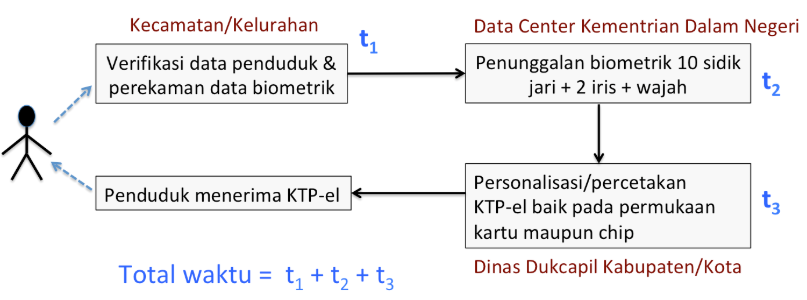
\includegraphics[width=12cm]{figures/probis.png}
	\caption{Gambaran Proses Bisnis Pembuatan KTP.}	
\end{figure}

\section{Analisis Dokumen }
Berikut analisis dokumen yang dibutuhkan pada pembuatan ktp sesuai dengan proses bisnis yang berlaku. Dari data tersebut terdapat banyak data yang redudansi. Oleh karena itu, kita melakukan analisis terhadap dokumen yang digunakan dalam proses pembuatan ktp dengan cara memisahkan atribut-atribut yang terdapat pada dokumen dan menganalisis atribut yang redudansi, agar kemudian kita bisa membuat design databasenya pada power designer tanpa ada lagi data yang redudansi. Pada tahap ini, kita harus bisa melihat data-data mana yang merupakan inti dari dokumen tersebut, dan data mana yang merupakan turunan dari dokumen lain. Setelah kita bisa menentukan atributnya, selanjutnya kita akan menentukan tipe data serta primary key-nya pada design yang akan kita buat di power designer.
\begin{table}
\caption{Tabel Atribut Dokumen}
\centering
\begin{tabular}{|c|c|c|}
\hline
\textbf{Akta Kelahiran}&\textbf{KK}&\textbf{Surat Pengantar}\\
\hline
No Akta&No KK&Nama Kabupaten\\
\hline
Kode Csi&Nama Kepala Keluarga&Nama Kecamatan\\
\hline
Warga Negara&Alamat&Nama Desa\\
\hline
Dari Daftar&RT/RW&No Surat\\
\hline
No STBLD&Desa/Kelurahan&Nama RT\\
\hline
Tempat Lahir&Kecamatan&Jabatan\\
\hline
Tanggal Lahir&Kabupaten/Kota&Alamat RT\\
\hline
Jam Kelahiran&Kode Pos&Nama Lengkap\\
\hline
Nama OrangTua&Provinsi&Jenis Kelamin\\
\hline
Urutan Anak&Nama Lengkap&NIK\\
\hline
Nama Ayah&NIK&Tempat Lahir\\
\hline
Nama Ibu&Jenis Kelamin&Tanggal Lahir\\
\hline
Tanggal Pembuatan Akta&Tempat Lahir&Pekerjaan\\
\hline
Ttd Dukcapil&Tanggal Lahir&Keperluan\\
\hline
Cap Dukcapil&Agama&Keterangan Lain\\
\hline
-&Pendidikan&Berlaku Mulai Tangga\\
\hline
-&Jenis Pekerjaan&Ttd\\
\hline
-&Status Perkawinan&Pembuatan Surat\\
\hline
-&Hubungan Keluarga&-\\
\hline
-&Kewarganegaraan&-\\
\hline
-&No.Pasport&-\\
\hline
-&No.KITAS/KITAP&-\\
\hline
-&Nama Ayah&-\\
\hline
-&Nama Ibu&-\\
\hline
-&Ttd&-\\
\hline
-&Cap Dukcapil&-\\
\hline
\end{tabular}
\end{table}

\begin{table}
\caption{Tabel Atribut Dokumen2}
\centering
\begin{tabular}{|c|c|}
\hline
\textbf{Form KTP}&\textbf{KTP}\\
\hline
Provinsi&Nama\\
\hline
Kabupaten/Kota&Tempat Lahir\\
\hline
Kecamatan&Tanggal Lahir\\
\hline
Kelurahan/Desa&Jenis Kelamin\\
\hline
Nama Lengkap&Golongan Darah\\
\hline
NIK&Alamat\\
\hline
Alamat Pemohon&RT/RW\\
\hline
Kelurahan/Desa&Provinsi\\
\hline
Kabupaten/Kota&Kota\\
\hline
Kecamatan&Kelurahan/Desa\\
\hline
Provinsi&Kecamatan\\
\hline
RT&Agama\\
\hline
RW&Status Perkawinan\\
\hline
Telepon&Pekerjaan\\
\hline
Alasan Permohonan&Kewarganegaraan\\
\hline
 & Foto\\
\hline
Jumlah Anggota Keluargal&Masa Berlaku\\
\hline
 &Ttd\\
\hline
-&Ttd\\
\hline
\end{tabular}
\end{table}

\begin{figure}[H]
	\centering
	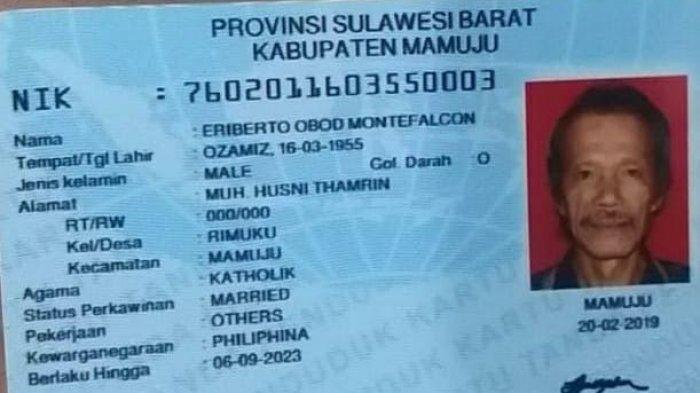
\includegraphics[width=16cm]{figures/ktp.jpg}
	\caption{KTP.}	
\end{figure}
\begin{figure}[H]
	\centering
	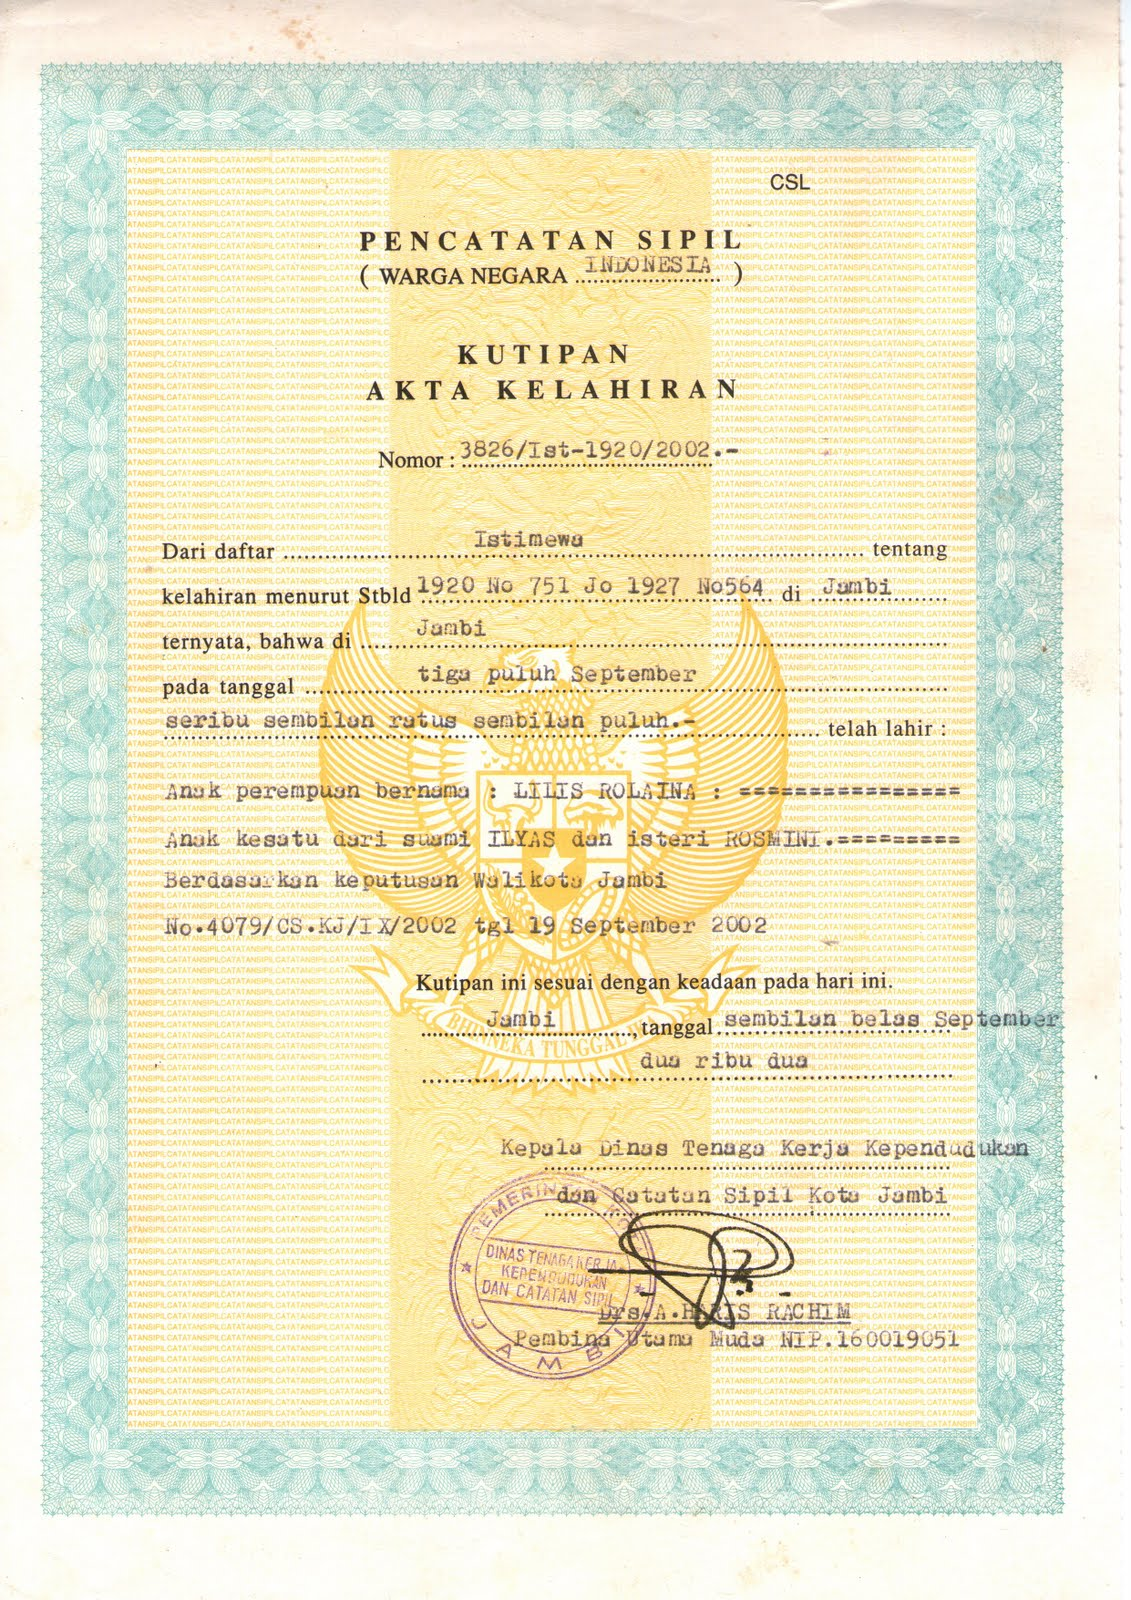
\includegraphics[width=16cm]{figures/akte.jpg}
	\caption{Akte Kelahiran.}	
\end{figure}
\begin{figure}[H]
	\centering
	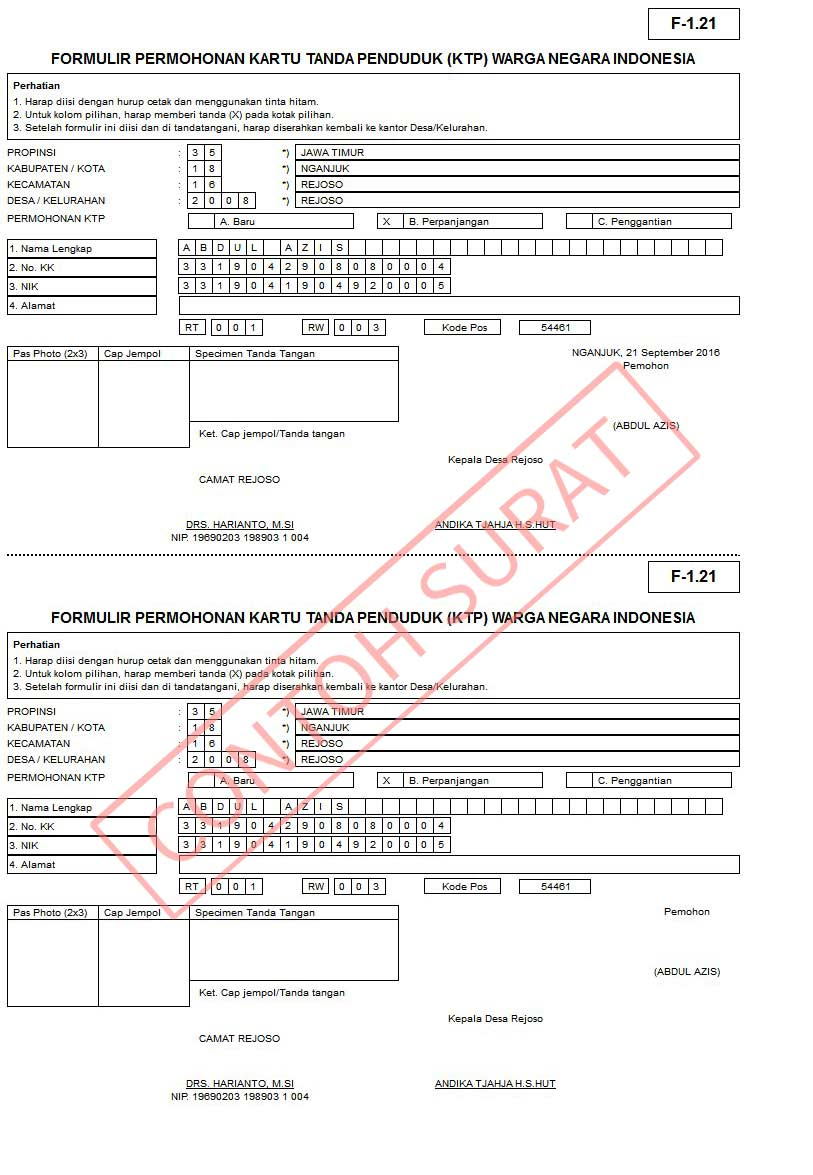
\includegraphics[width=16cm]{figures/form.jpg}
	\caption{Formulir KTP.}	
\end{figure}
\begin{figure}[H]
	\centering
	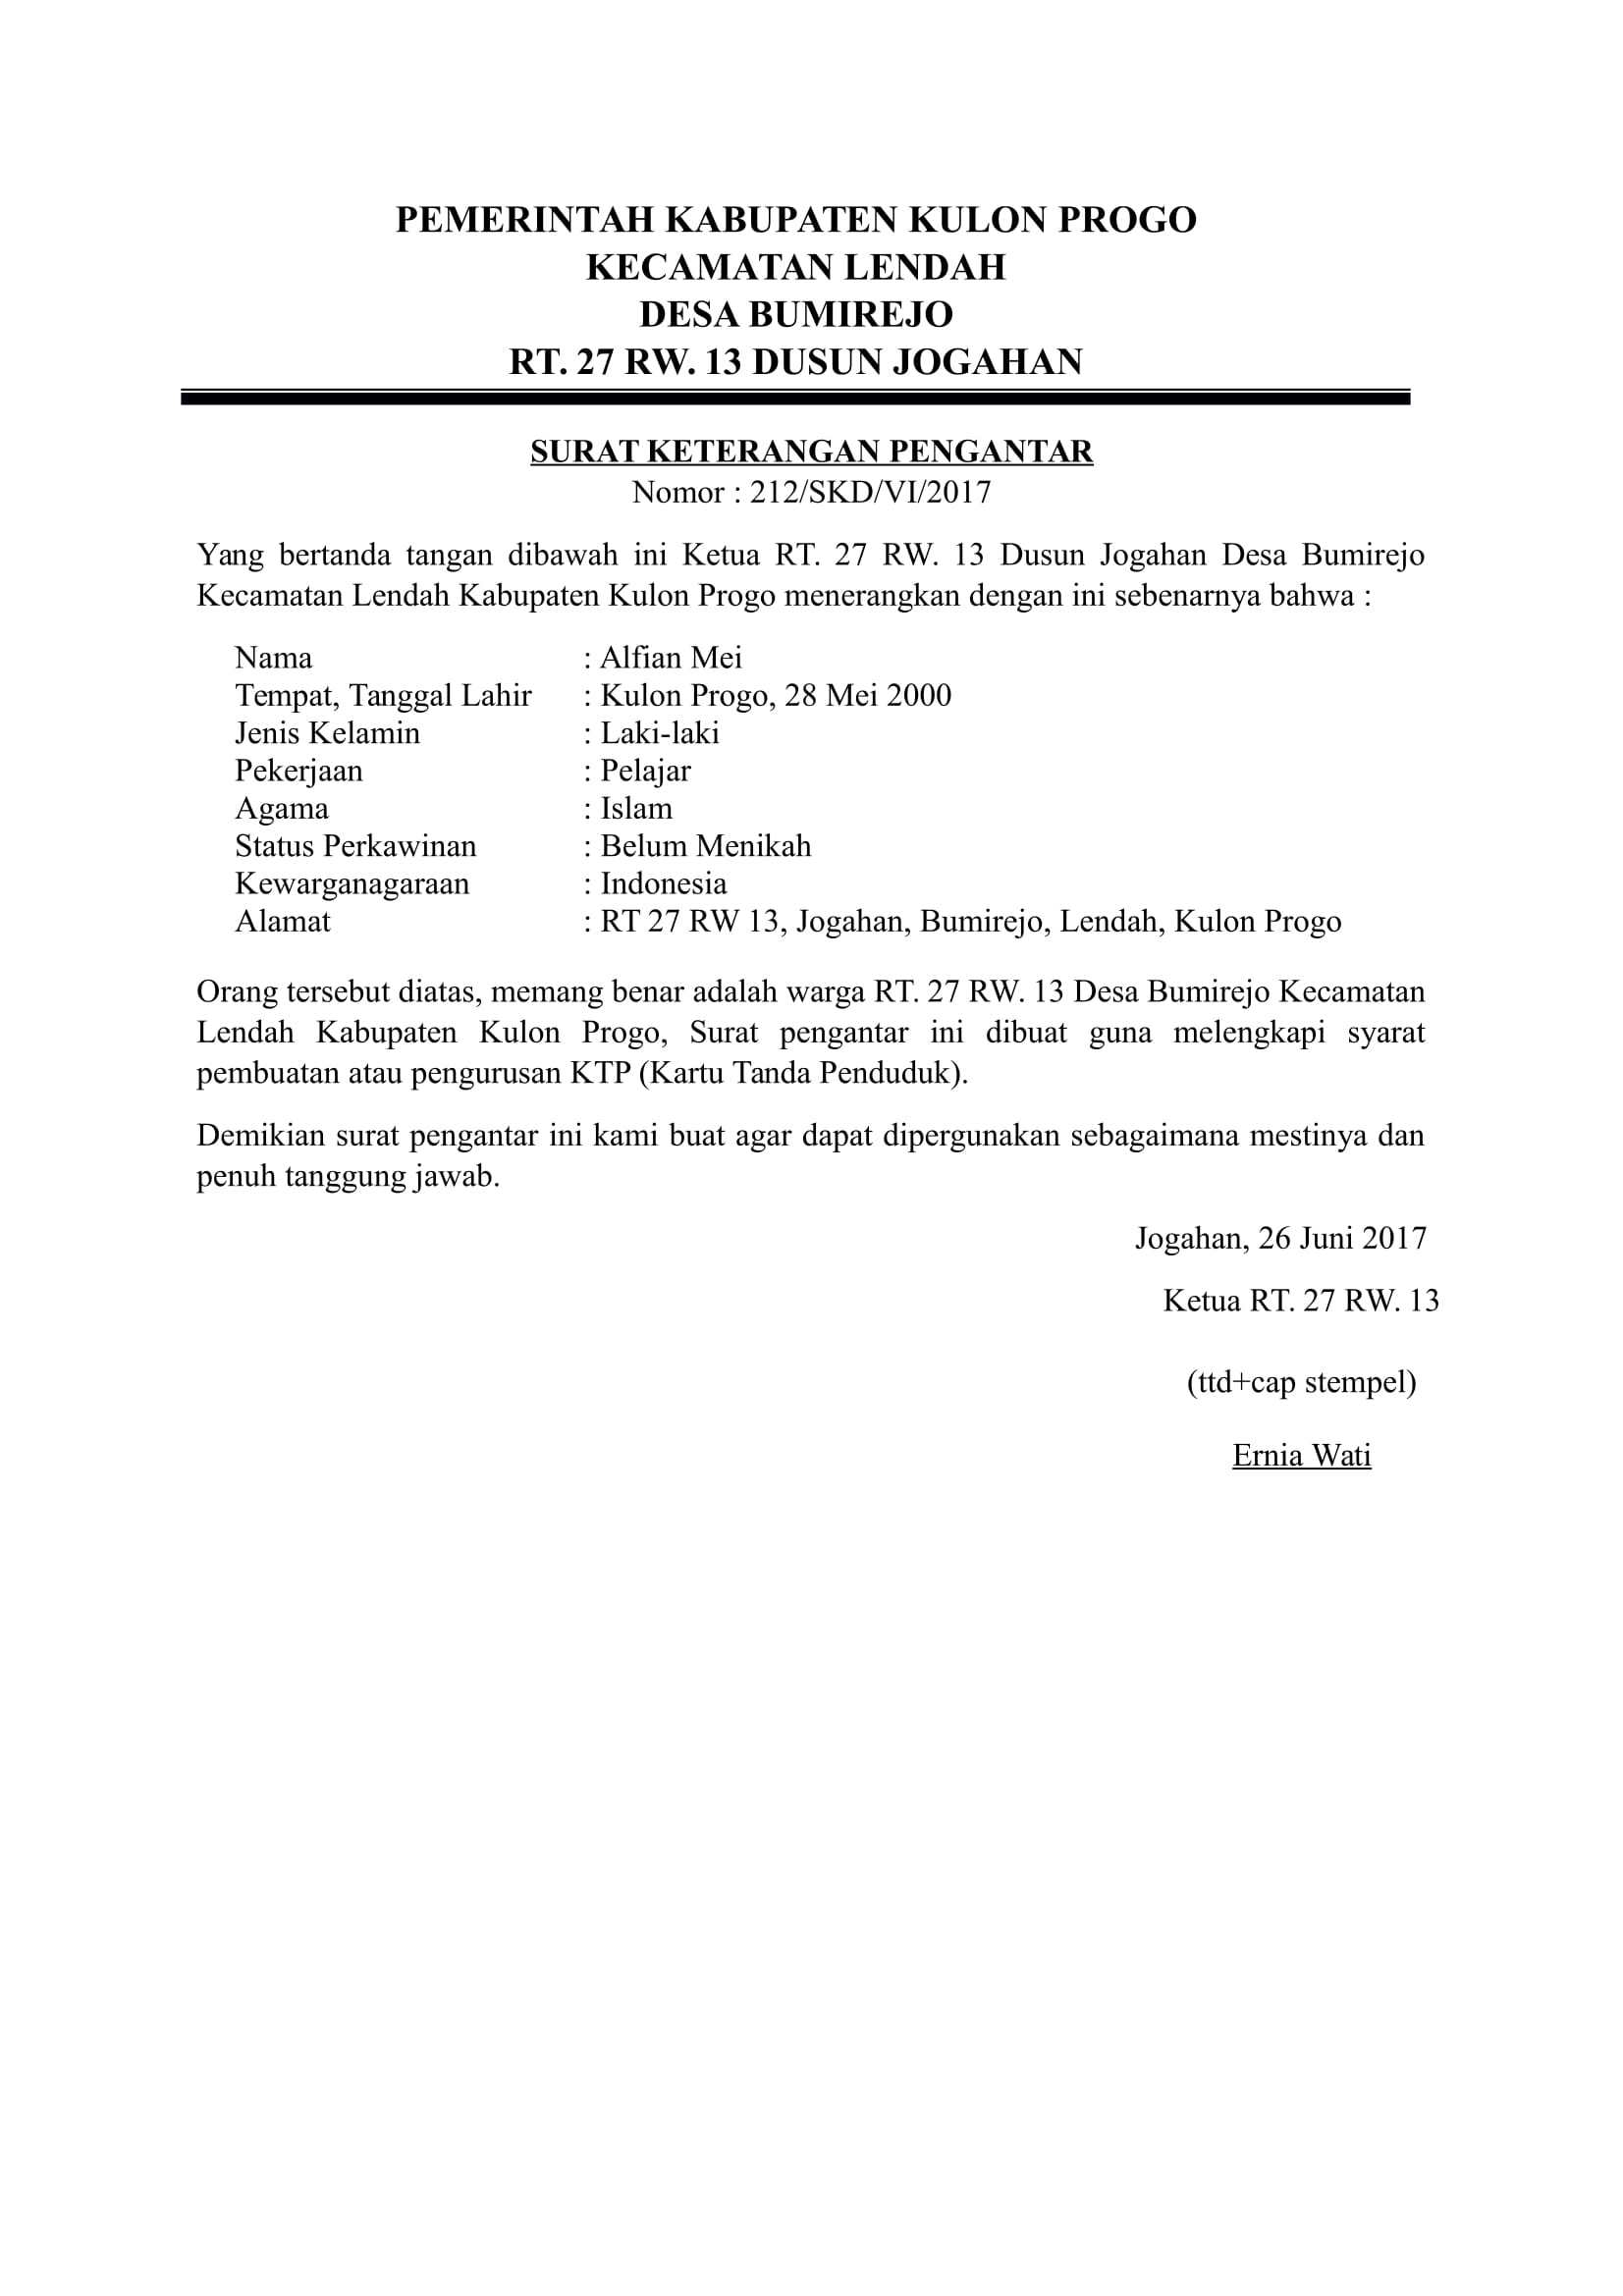
\includegraphics[width=16cm]{figures/pengantar.jpg}
	\caption{Surat Pengantar.}	
\end{figure}
\begin{figure}[H]
	\centering
	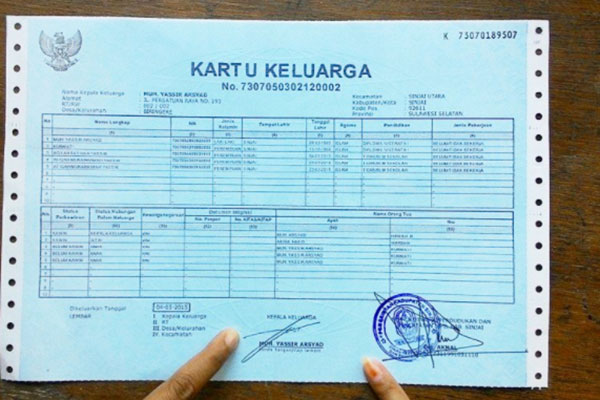
\includegraphics[width=16cm]{figures/kk.jpg}
	\caption{Kartu Keluarga.}	
\end{figure}
